\documentclass[sokoban_generation_thesis.tex]{subfiles}

Kluczowe z~punktu widzenia metody PDB jest dobranie odpowiedniej sekwencji $[\cdot]$. Autorzy metody, analizując jej wyniki, wyznaczyli sześć wariantów opartych na~dwudziestu różnych sekwencjach $[\cdot]$. W~niniejszej pracy postanowiono przebadać trzy warianty o~najlepszych wynikach, z~których każdy oparty był na~czterech sekwencjach. Takie podejście pozwala na~bardziej kompleksowe zbadanie skuteczności metody w~różnych konfiguracjach. Poniższe opisy badanych wariantów uwzględniają wielkości wzorców $k$ z~przedziału $[2, 5]$.

\begin{enumerate}
	\item Wariant prosty -- nie korzysta z~funkcji nowości. Przyjęte sekwencje są~postaci $\left[kC, h^{PDB_k}\right]$. %C
	\item Wariant nowości -- korzysta z~funkcji nowości. Przyjęte sekwencje są~postaci $\left[w(h^{PDB_k}), h^{PDB_k}\right]$. %D
	\item Wariant złożony -- korzysta z~funkcji nowości oraz heurystyki konfliktów. Przyjęte sekwencje są~postaci $\left[w(h^{PDB_k}), kC, h^{PDB_k}\right]$. %F
\end{enumerate}


\begin{figure}[h!]
	\centering
	\begin{subfigure}[b]{0.55\textwidth}
		\centering
		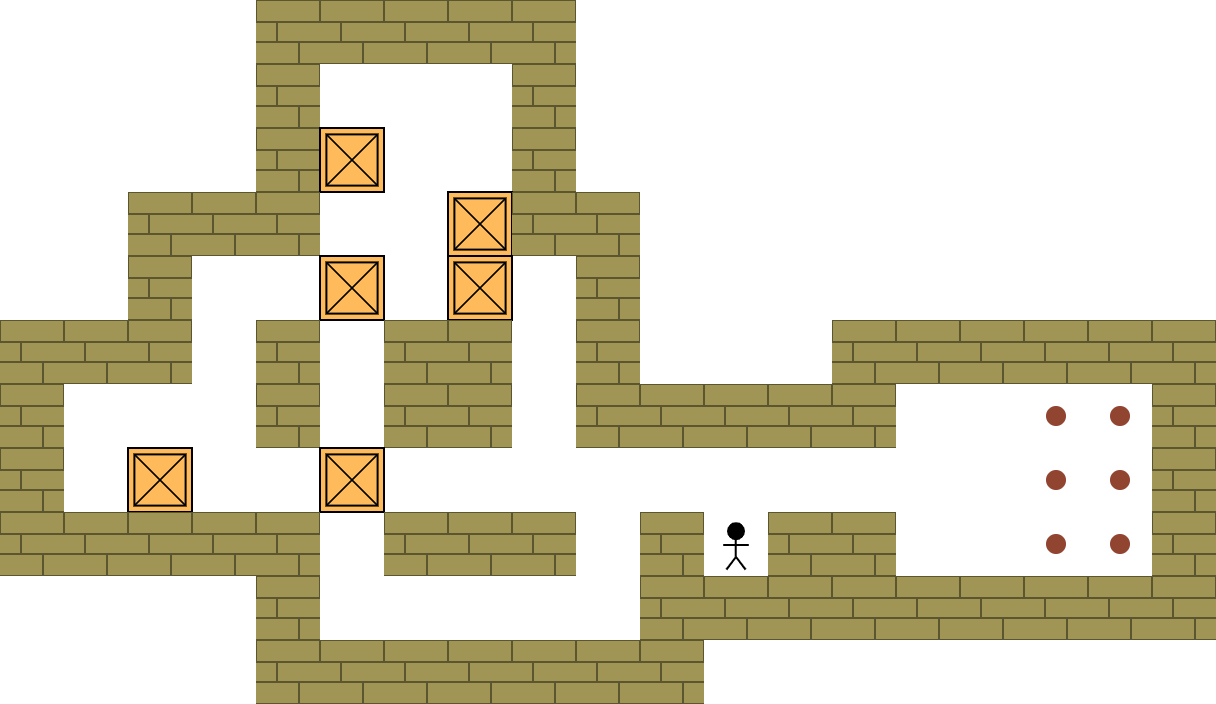
\includegraphics[width=0.8\textwidth]{board_pdb_source1}
		\caption{Plansza ze~zbioru\textit{XSokoban}}
	\end{subfigure}
	\hspace{0.02\textwidth}
	\begin{subfigure}[b]{0.35\textwidth}
		\centering
		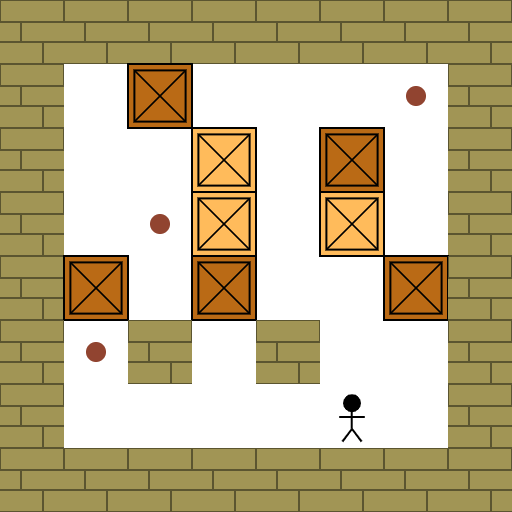
\includegraphics[width=0.7\textwidth]{board_pdb_source2}
		\caption{Plansza ze~zbioru \textit{SokEvo}}
	\end{subfigure}
	\caption{Przykładowe plansze z~użytych zbiorów}
	\label{rys:sample_from_sets}
\end{figure}

Badania autorów metody PDB zostały również poszerzone o~dodatkowy zbiór plansz. Poza zbiorem \textit{XSokoban} złożonym z~$90$ plansz, postanowiono wykorzystać zbiór \textit{SokEvo}, na~który składa się $107$ poziomów \cite{sok_wiki}. Zasadnicza różnica między tymi zbiorami polega na~tym, że~żaden z~poziomów w~pierwszym z~nich nie jest kształtu prostokąta, zaś w~drugim -- wszystkie. Przykładowe plansze z~obu zbiorów wraz odpowiadającymi im~wynikami metody ukazano na~rys.~\ref{rys:sample_from_sets} i~\ref{rys:results_from_sets}.

\begin{figure}[h!]
	\centering
	\begin{subfigure}[b]{0.55\textwidth}
		\centering
		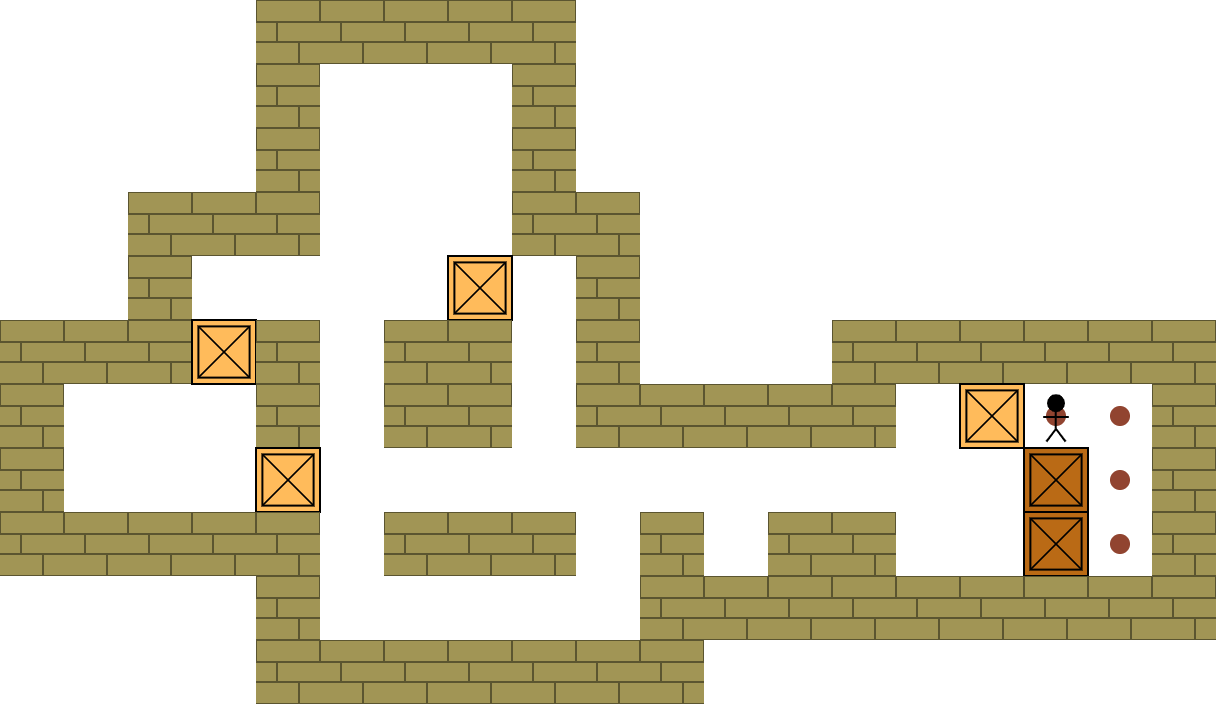
\includegraphics[width=0.8\textwidth]{board_pdb_result1}
		\caption{Plansza ze~zbioru \textit{XSokoban}}
	\end{subfigure}
	\hspace{0.02\textwidth}
	\begin{subfigure}[b]{0.35\textwidth}
		\centering
		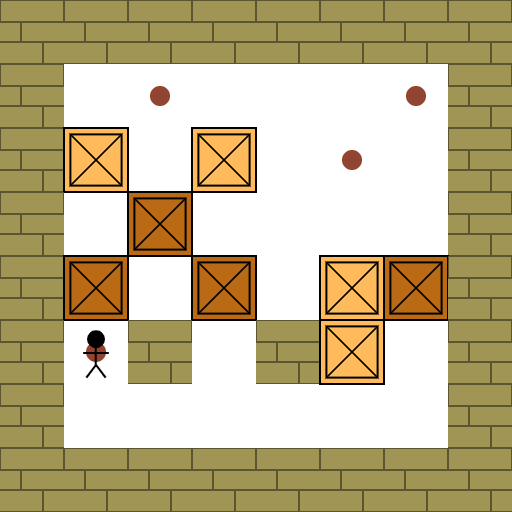
\includegraphics[width=0.7\textwidth]{board_pdb_result2}
		\caption{Plansza ze~zbioru \textit{SokEvo}}
	\end{subfigure}
	\caption{Przykładowe wyniki metody PDB oparte na~planszach z~rys.~\ref{rys:sample_from_sets}}
	\label{rys:results_from_sets}
\end{figure}


\subsection{Wydajność czasowa} \label{subs:pdb_time}
W celu zbadania wydajności czasowej metody PDB, postanowiono wyznaczyć uśrednione wartości heurystyk $h^{PDB_2}-h^{PDB_5}$ dla różnych czasów działania. Z~reguły obserwuje się około $60\%$ wzrost na~przestrzeni pierwszych dziesięciu minut działania, potem tempo poprawy generowanych poziomów spada. Oceny poziomów ze~zbioru \textit{SokEvo} były na~ogół niższe, najpewniej z~uwagi na~mniej skomplikowane kształty poziomów. Analizy wskazały również na~to, że~wariant nowości radził sobie lepiej niż wariant złożony w~kwestii heurystyk baz danych wzorców.

\begin{figure}[h!]
	\centering
	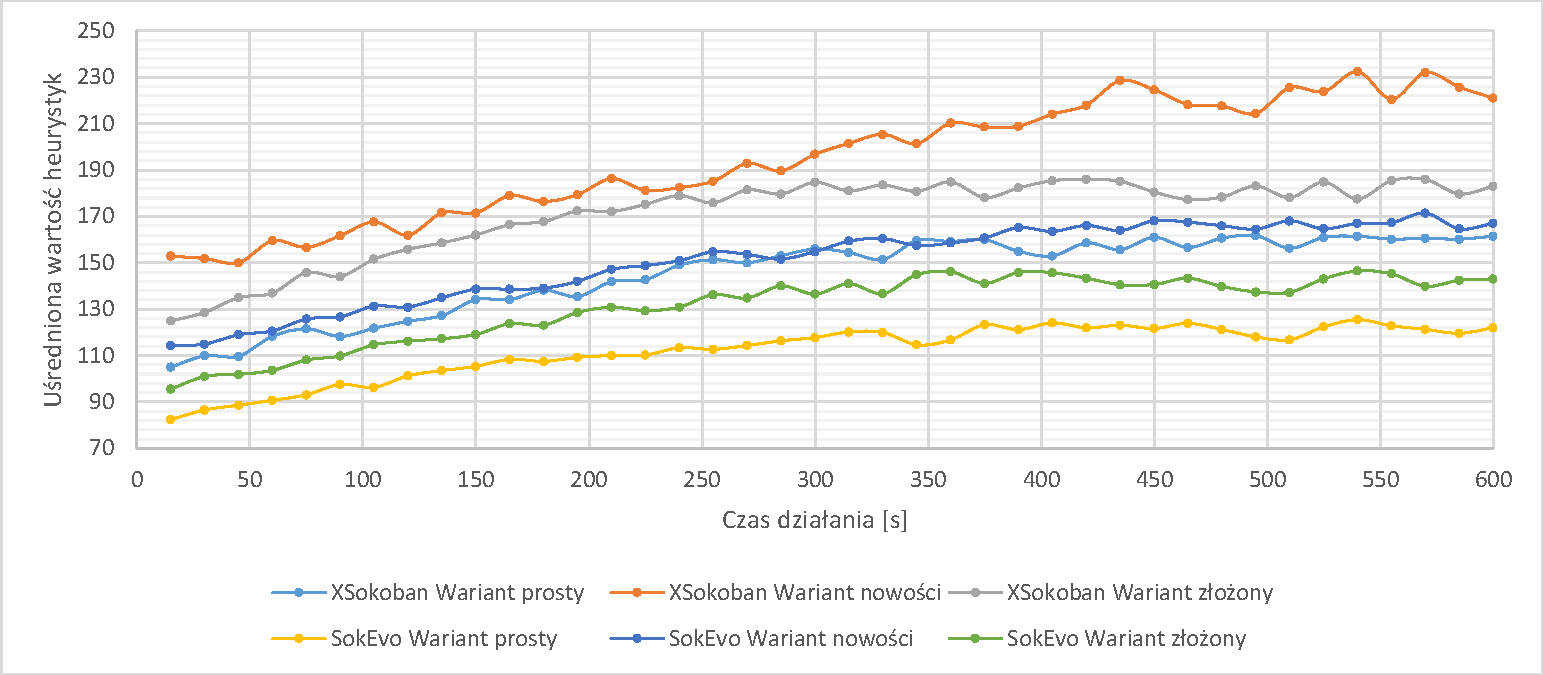
\includegraphics[width=0.9\textwidth]{pdb_heurs_time}
	\caption{Zależność wartości heurystyk od~czasu pracy}
	\label{rys:pdb_heurs_time}
\end{figure}

Metoda PDB zaczyna pracę z~rozwiązaną planszą i~wraz z~kolejnymi iteracjami przeszukiwania grafu, zmienia ustawienia pudeł oraz gracza, zmniejszając tym samym liczbę pudeł na~polach docelowych. W~ramach analizy wydajności czasowej metody, postanowiono również zbadać jak wygląda zależność czasu od~stosunku pudeł niestojących na~polach docelowych do~wszystkich pudeł. Tak opisany stosunek określa się dalej skutecznością, która dla planszy rozwiązanej ma~wartość $0\%$, a~dla planszy bez pudeł na~polach docelowych -- $100\%$. Wykres na~rys.~\ref{rys:pdb_solved_boxes_time} prezentuje dane uśrednione ze~wszystkich eksperymentów zaprezentowanych w~niniejszym podrozdziale. Jak widać, w~celu uzyskania skuteczności na~poziomie $50\%$, wystarczy około $15$ sekund, a~dla prawie pełnej gwarancji uzyskania poziomu o~nietrywialnym rozkładzie pudeł -- ponad $15$ minut.

\begin{figure}[h!]
	\centering
	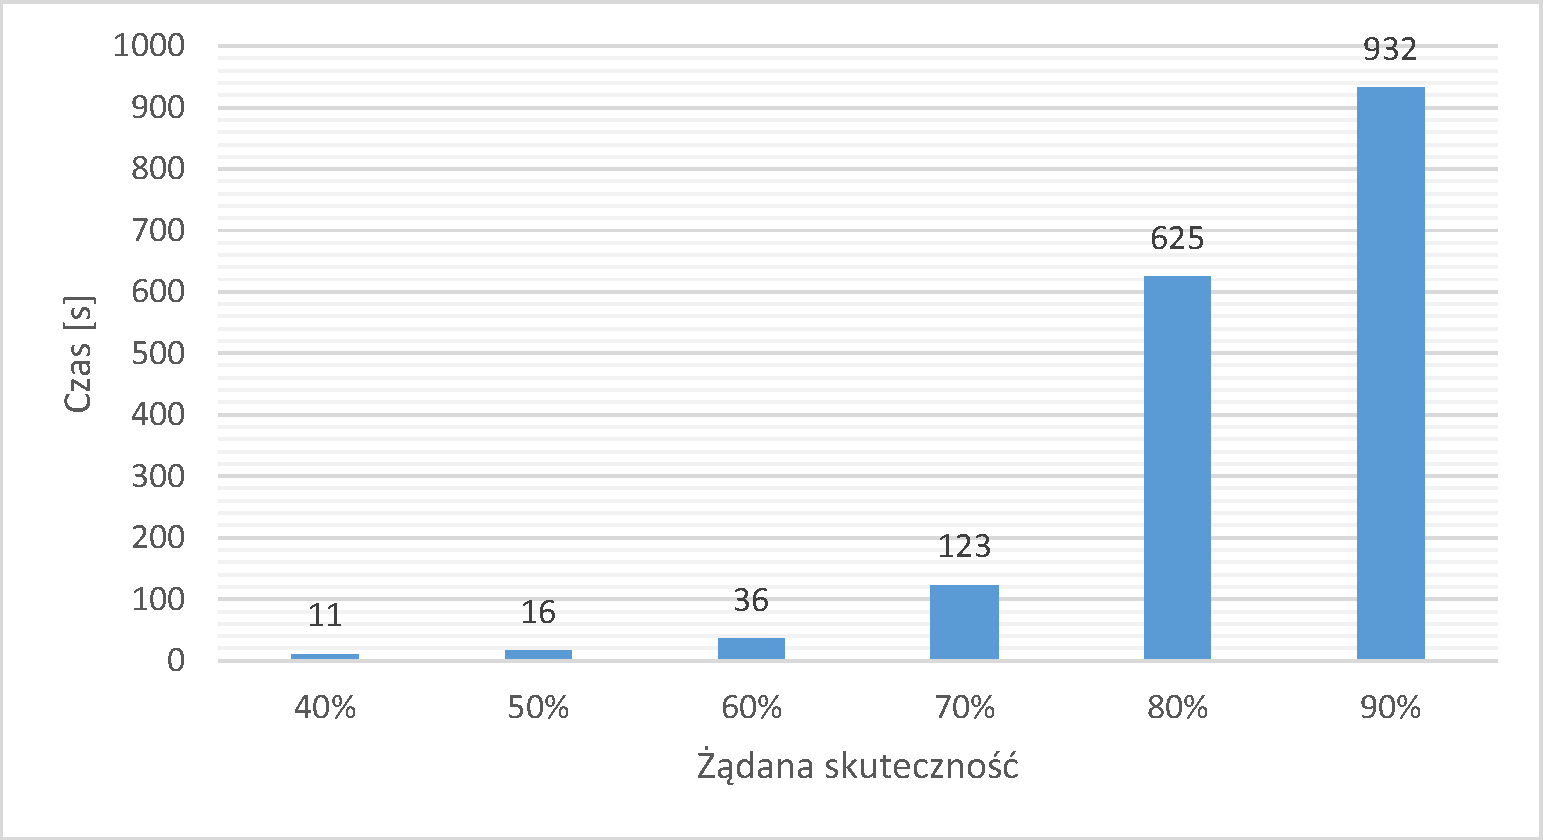
\includegraphics[width=0.8\textwidth]{pdb_czas_needed}
	\caption{Zależność czasu od~żądanej skuteczności}
	\label{rys:pdb_solved_boxes_time}
\end{figure}

\subsection{Wydajność pamięciowa}
Algorytm $\beta$ opisany dokładnie w~p.~\ref{subs:pdb_method_description} korzysta z~kolejki priorytetowej, w~której przetrzymuje analizowane stany (plansze). Zaobserwowano, że~wraz z~czasem działania metody jej zapotrzebowania pamięciowe rosną liniowo. Wyniki analiz zaprezentowano na~rys.~\ref{rys:pdb_ram}. Jak widać, $10$ minut działania metody jest związane ze~zużyciem prawie $5$ GB~pamięci.

\begin{figure}[h!]
	\centering
	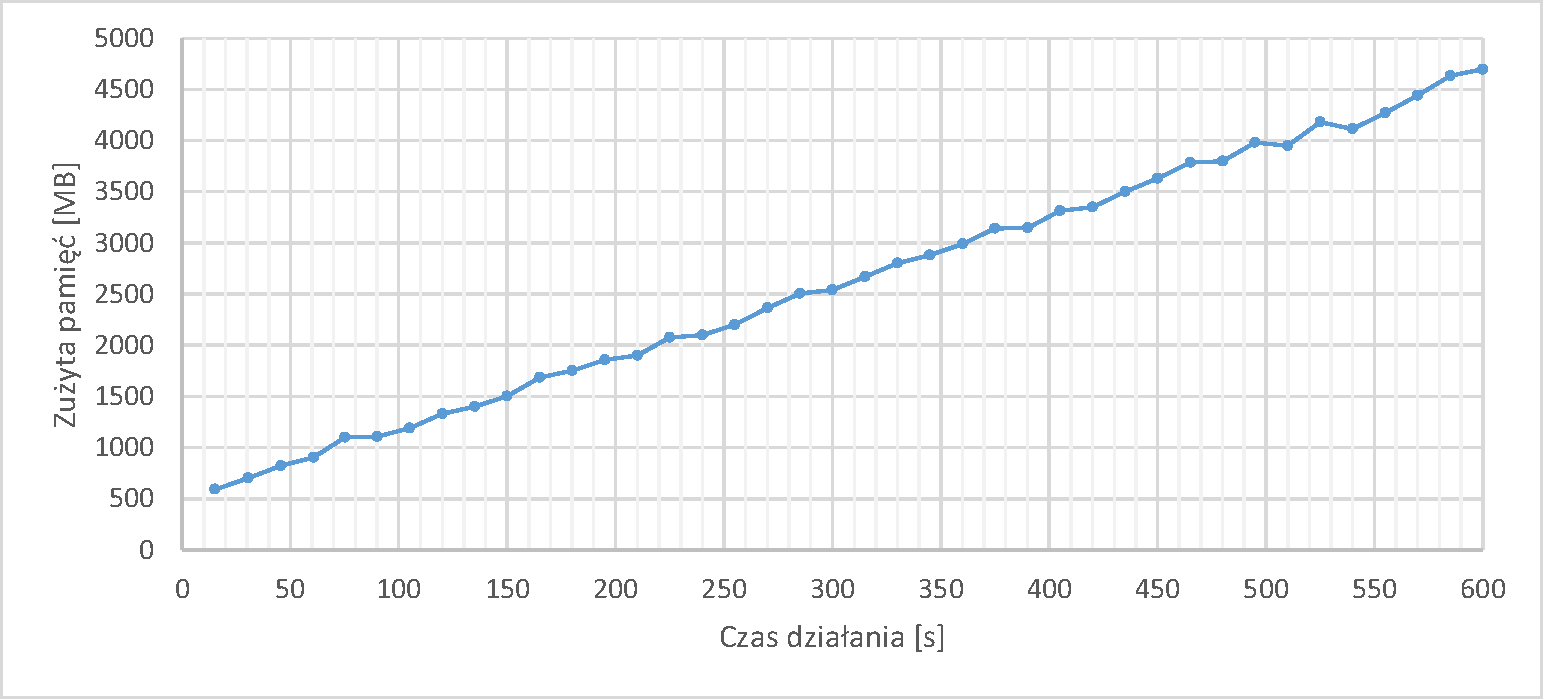
\includegraphics[width=0.8\textwidth]{pdb_ram}
	\caption{Zależność zużytej pamięci od~czasu pracy}
	\label{rys:pdb_ram}
\end{figure}

\subsection{Funkcja nowości i~liczba konfliktów}
Poza wartościami heurystyk $h^{PDB}$ należy też zbadać wartości heurystyki konfliktów $kC$, która również służy wycenie generowanych poziomów. W~tym celu zaprezentowane zostały rys.~\ref{rys:pdb_heur_pdb} i~\ref{rys:pdb_heur_conf}, obrazujące wyniki tych badań. Jak widać, prawie w~każdym przypadku wariant prosty generował plansze o~najniższych wartościach heurystyk. Istotną obserwacją jest fakt, że~wariant nowości generuje plansze o~wyższych wartościach heurystyk baz danych wzorców, ale to~wariant złożony produkuje plansze o~większej liczbie konfliktów. Wynika to~z~konstrukcji sekwencji $[\cdot]$ wariantu złożonego, który uwzględnia liczbę konfliktów w~trakcie przeszukiwania kolejnych stanów. Praktycznym wnioskiem, jaki należałoby wysnuć z~przedstawionej analizy jest to, że~wariant nowości skupia się na~długości rozwiązującej ścieżki, podczas gdy wariant złożony -- na~liczbie zależności między pudłami.

\begin{figure}[h!]
	\centering
	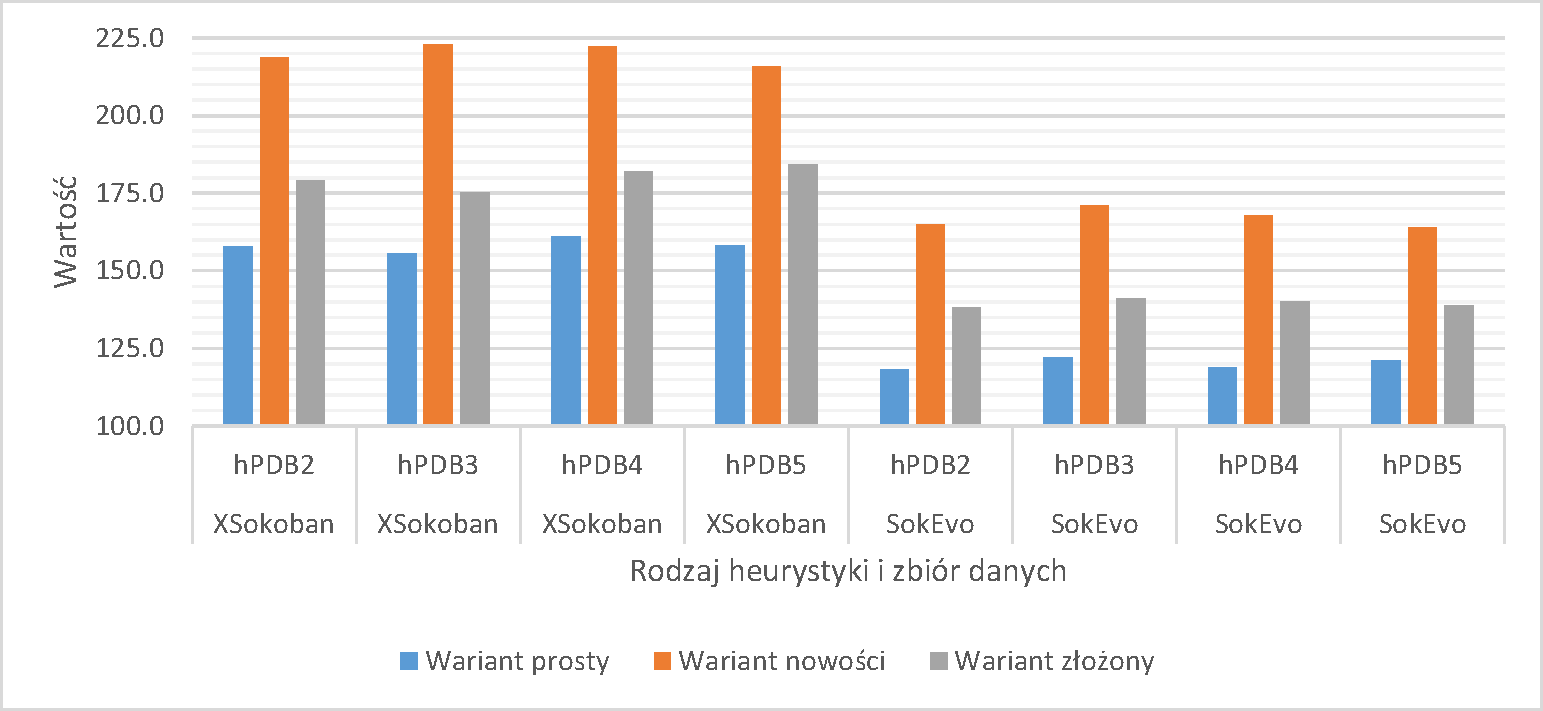
\includegraphics[width=0.85\textwidth]{pdb_heur_pdb}
	\caption{Wartości heurystyk baz danych wzorców}
	\label{rys:pdb_heur_pdb}
\end{figure}

\begin{figure}[h!]
	\centering
	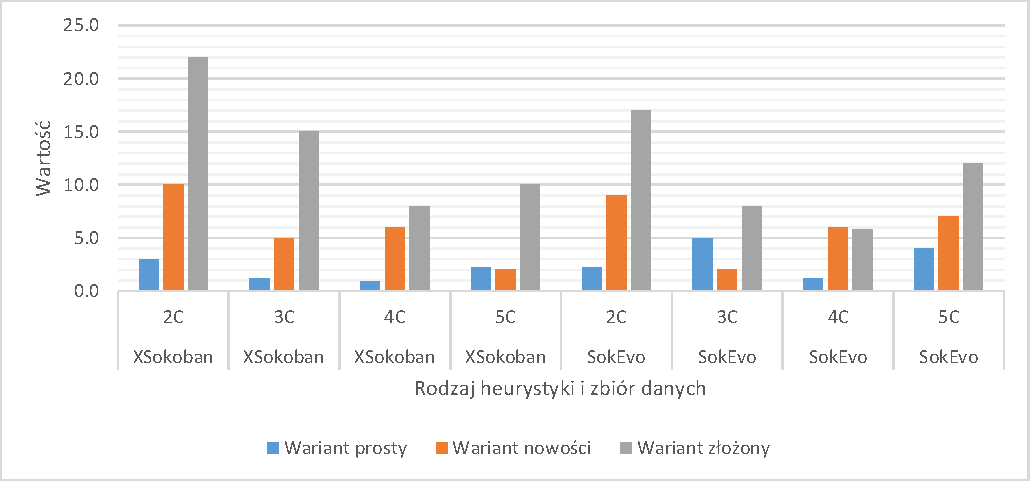
\includegraphics[width=0.85\textwidth]{pdb_heur_conf}
	\caption{Wartości heurystyki konfliktów}
	\label{rys:pdb_heur_conf}
\end{figure}